\documentclass[a4paper]{article}

\usepackage[left=1cm, right=1cm, top=2cm, bottom=2cm]{geometry}

\usepackage[utf8]{inputenc}
\usepackage[russian]{babel}

\usepackage[colorlinks,allcolors=black]{hyperref}

\usepackage{amsmath}

\usepackage{graphicx}

\usepackage{array}
\newcolumntype{P}[1]{>{\centering\arraybackslash}p{#1}}
\newcolumntype{M}[1]{>{\centering\arraybackslash}m{#1}}


\usepackage{listings}
\usepackage{xcolor}
\lstset { %
    language=C++,
    backgroundcolor=\color{black!5}, % set backgroundcolor
    basicstyle=\footnotesize,% basic font setting
}



\begin{document}

\begin{center}
\Large{\textbf{Учет инерционной керровской нелинейности}}
\end{center}

\noindent Как известно, инерционная керровская нелинейность рассчитывается через свертку 
\begin{equation}
\label{eqn:delta_n_k}
\Delta n_{inertial} (\mathbf{r}, t) = g n_2 \int\limits_{0}^{+\infty} H(\tau) I(\mathbf{r}, t - \tau) d\tau,
\end{equation}
с затухающим гармоническим ядром (Рис. 1):
\begin{equation}
\label{eqn:h_t}
H(t) = \Theta(t) \frac{1 + \Omega_R^2 \tau_k^2}{\Omega_R \tau_k^2} \sin(\Omega_R t) \exp \{ -t/\tau_k \}
\end{equation}
и $g$ -- весовой коэффициент, $H(t)$ -- ядро свертки, $\Theta(t)$ -- ступенчатая функций Хевисайда, $\Omega_R$ -- вращательная частота молекул, $\tau_k$ -- характерное время отклика. 

\begin{figure}[h]
\begin{center}
\begin{tabular}{M{10cm}}
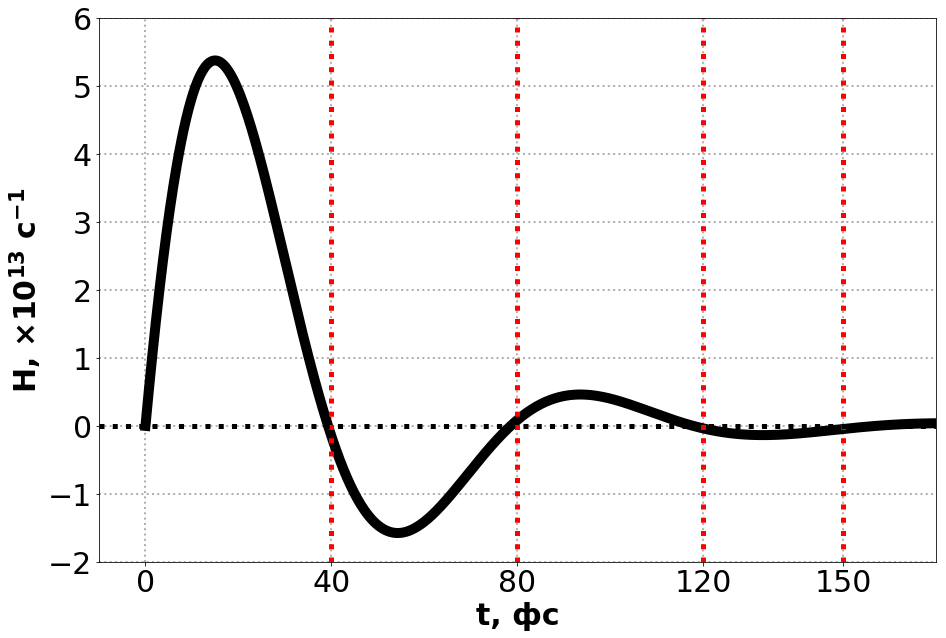
\includegraphics[width=\linewidth]{images/convolution.png}
\end{tabular}
\begin{minipage}{0.7\textwidth}
\caption{Ядро свертки, описывающей инерционную керровскую нелинейность \eqref{eqn:delta_n_k}. Красными пунктирными линиями изображены некоторые нули функции.}
\end{minipage}
\label{pic:convolution_h}
\end{center}
\end{figure}

\begin{figure}[h]
\begin{center}
\begin{tabular}{M{10cm}}
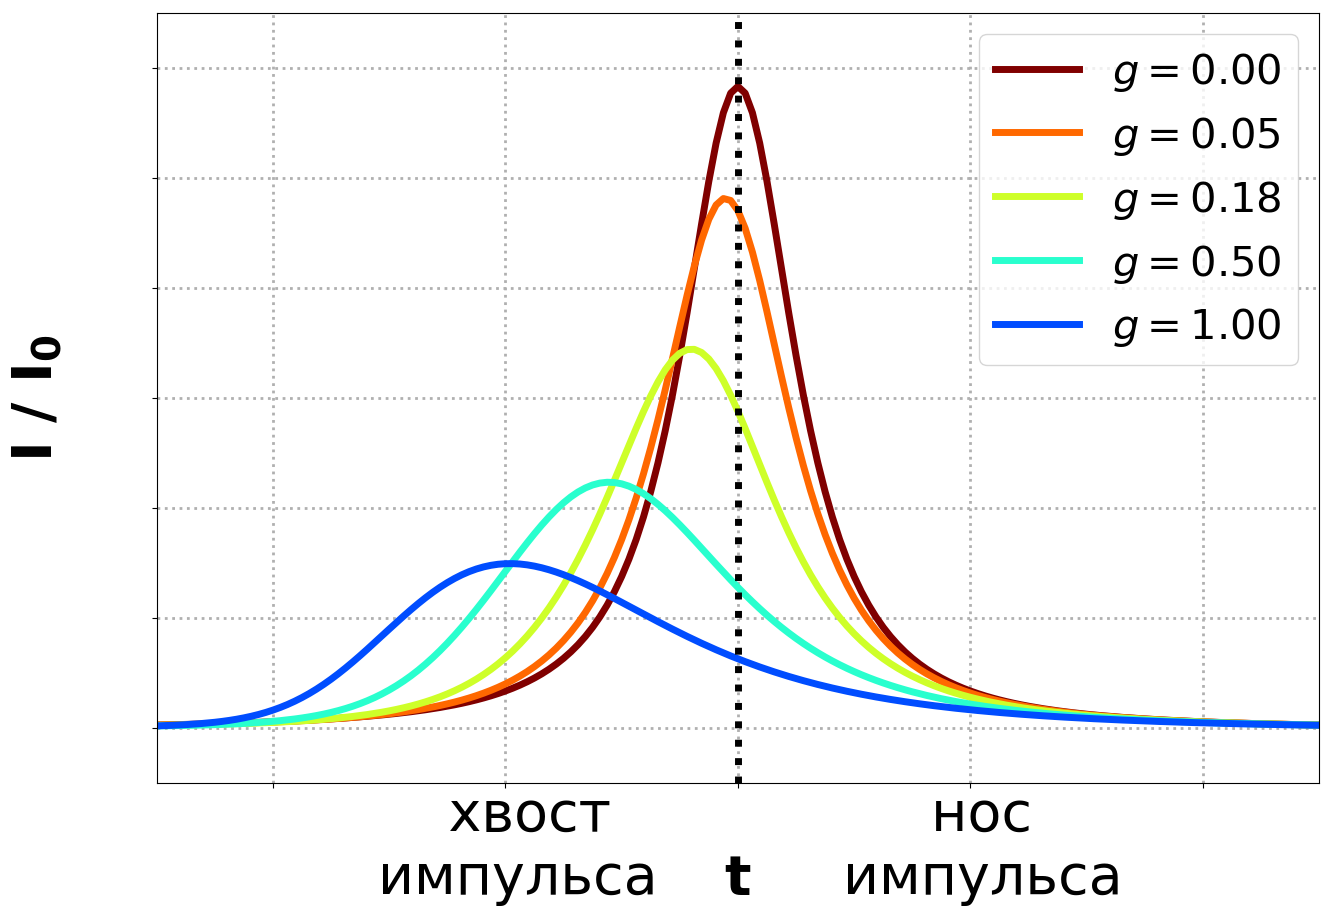
\includegraphics[width=\linewidth]{images/kerr_inertial_g.png}
\end{tabular}
\begin{minipage}{0.7\textwidth}
\caption{Временные профили интенсивности при самофокусировке спектрально-ограниченного гауссова импульсного пучка для разного вклада инерционной керровской нелинейности $g$. Пунктирной линией показан центральный временной слой.}
\end{minipage}
\label{pic:kerr_inertial_g}
\end{center}
\end{figure}

На Рис. 2 показаны временные профили интенсивности при самофокусировке импульса для разных $g$. Видно, что при увеличении $g$ положение пиковой интенсивности смещается к хвосту импульса, а значение интенсивности уменьшается. Случаи $g=0$ (красная кривая) и $g=1$ (синяя кривая) являются вырожденными и соответствуют приближениям полностью мгновенной и полностью инерционной керровской нелинейности соответственно. При $g=0$ отклик среды лишен запаздывания и пиковая интенсивность расположена строго в центральном временном слое. При $g=1$ инерционность среды приводит к максимальному смещению пиковой интенсивности. Степень смещения зависит от параметров инерционности и определяется выражением \eqref{eqn:h_t}.



Взятие свертки имеет квадратичную алгоритмическую сложность. Одним из способов ускорения расчетов в этом случае является ограничение ядра свертки временным окном $\Delta_t$. Необходимо выбрать такое минимальное временное окно, которое не вносило бы существенных изменений в самофокусировку по сравнению с полным расчетом свертки.


Поскольку ядро осциллирует, среди возможных временных окон $\Delta_t$ будем рассматривать только те, что соответствуют нулям функции \eqref{eqn:h_t}. Использование других возможных окон, при которых осцилляция обрывается в произвольном месте, выглядит неестественно с точки зрения физического смысла, поэтому рассмотрим только следующие значения $\Delta_t$: 40, 80, 120 и 150 фс (Рис. 1). 
\begin{figure}[h]
\begin{center}
\begin{tabular}{M{10cm}}
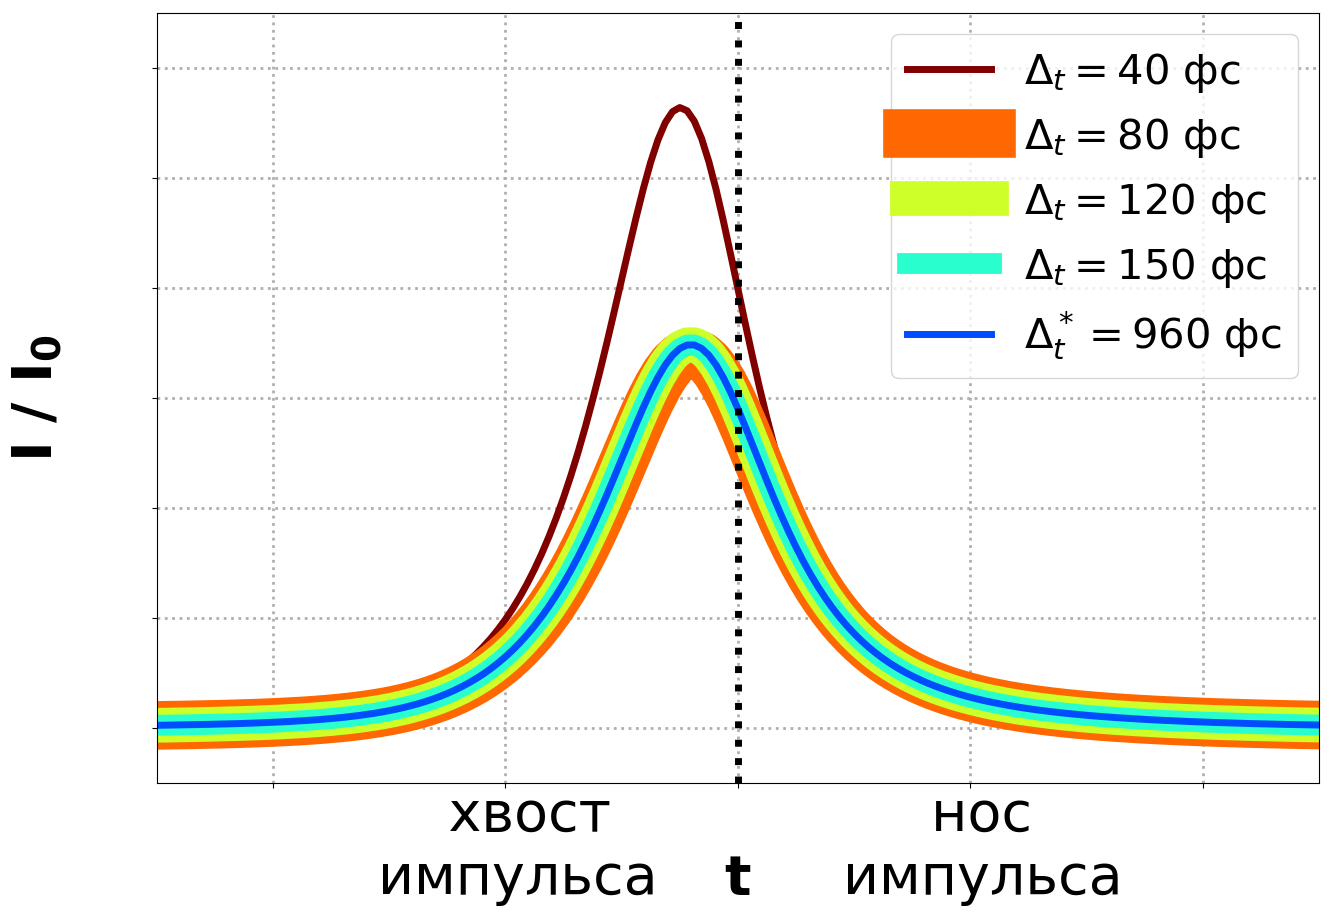
\includegraphics[width=\linewidth]{images/kerr_inertial_w.png}
\end{tabular}
\begin{minipage}{0.7\textwidth}
\caption{Временные профили интенсивности при самофокусировке спектрально-ограниченного гауссова импульсного пучка для разных окон свертки $\Delta_t$ при моделировании \eqref{eqn:h_t}. Пунктирной линией показан центральный временной слой.}
\end{minipage}
\label{pic:kerr_inertial_w}
\end{center}
\end{figure}
На Рис. 3 изображены временные профили интенсивности при самофокусировке с разными временными окнами $\Delta_t$. Окно $\Delta_t^* = 960$ фс соответствует полному расчету свертки. Видно, что при $\Delta_t = 40$ фс профиль довольно сильно отличается от случая $\Delta_t^*$, в то время как остальные величины окон находятся с ним в хорошем согласии. Таким образом, минимальное значение окна $\Delta_t$, при котором нет существенных отличий от полного расчета свертки, составляет $\Delta_t = 80$ фс, что соответствует учету одной полной осцилляции ядра. 

Строго говоря, приведенная оценка справедлива только для процесса самофокусировки. Для распространения рассуждений на общий случай филаментации, можно было бы ввести метрику отличия расчетов друг от друга (например, $L_1$-мера для распределения интенсивности на каждом шаге по $z$), посчитать свертку с окном, равным величине сетки, а затем плавно уменьшать $\Delta_t$. Пограничную величину окна, при котором отличие еще не так существенно, можно принять за искомую оптимальную величину $\Delta_t^{opt}$. Думаю, что $\Delta_t^{opt} \simeq 150$ фс.

Заметим, что наличие оператора волновой нестационарности $\hat{T}$, стоящего в нелинейном волновом уравнении перед керровской нелинейностью, приводит к тому, что инерционная нелинейность должна также учитываться в поправке с производной по $t$:
\begin{equation}
\begin{aligned}
A^{n+1} = A^{n} \exp \biggl\{\biggl[
&R_{inst} I_{s} + R_{instT} \frac{I_{s} - I_{s-1}}{h_t} +\\
+&R_{iner} \Bigl( H(t_s) \otimes I_s \Bigr) + R_{inerT} \frac{ H(t_s) \otimes I_s - H(t_{s-1}) \otimes I_{s-1}}{h_t} +\\
+&R_{ion} N_{e_s} + R_{ionT} \frac{N_{e_s} - N_{e_{s-1}}}{h_t} +\\
+&R_{B} N_{e_s} + R_{BT} \frac{N_{e_s} - N_{e_{s-1}}}{h_t}+\\
+&\frac{\alpha + \beta}{2}
\biggr] h_z \biggr\}
\end{aligned}
\end{equation}

Программная реализация расчета инерционной керровской нелинейности на языке С++ методом свертки с окном представлена ниже.

\noindent Необходимые константы:
\begin{lstlisting}

...

//Kerr
const double g = 0.18;
const double OmegaR = 8e13; // [s^-1]
const double tau_k = 32e-15; // [s]
const double R_H = (1 + sqr(OmegaR * tau_k)) / (OmegaR * sqr(tau_k));

...

std::complex<double> R_inertial = -_Complex_I * k0 * g * n2 * I0 * R_H * dt / n0;
double R_inertialT = -k0 * g * n2 * I0 * R_H * dt / (n0 * omega0);


...

\end{lstlisting}

\noindent Функция ядра свертки:
\begin{lstlisting}
...

double H(double t) {
	return sin(OmegaR * t) * exp(-t / tau_k);
}

...
\end{lstlisting}

\noindent Часть цикла учета нелинейностей (распараллелен по пространственной координате $r$), описывающая инерционную керровскую нелинейность:
\begin{lstlisting}
...

#pragma omp parallel 
{
#pragma omp for 
	for (int idx_r = 0; idx_r < Nr; ++idx_r) {
		
		...		
		
		double conv = 0.0;
		double conv_prev = 0.0;
		for (int idx_t = 1; idx_t < Nt; ++idx_t) {	
			//KerrInertial
			
			conv = 0.0;
		
			double conv_length = 80e-15; // [s]
			int conv_max = (int)(conv_length / dt);
			int tau_max = idx_t;
			if (idx_t > conv_max) tau_max = conv_max;

			int idx_tau = 0;
			while (idx_tau <= tau_max) {
				conv += H(idx_tau * dt) * norm(A[idx_r * Nt + (idx_t - idx_tau)]);
				++idx_tau;
			}
			
			...
			
std::complex<double> NonlinAmpPhase =
					(
					  ...
					+ R_inertial * conv 
					+ R_inertialT * (conv - conv_prev) / dt
					...
					) * *dz;

				A[idx_r * Nt + idx_t] *= exp(NonlinAmpPhase);	
				
			...
			
			conv_prev = conv;		
			
			...
			
\end{lstlisting}

\end{document}